\documentclass[12pt,letterpaper]{article}
\usepackage[margin=0.7in,headheight=16pt,headsep=16pt,footskip=25pt]{geometry}
\usepackage[T1]{fontenc}
\usepackage{lmodern}
\usepackage{tikz}
\usetikzlibrary{arrows.meta}
\usepackage{fancyhdr}
\renewcommand{\familydefault}{\sfdefault}
\pagestyle{fancy}
\fancyhf{}
\fancyhead[L]{\small Week 5 / Tower-city return visits / Grades 2--5}
\fancyfoot[L]{\small Bellingham Math Circle / Week 5 / F05-RV-v1}
\fancyfoot[R]{\small\thepage}
\renewcommand{\headrulewidth}{0.3pt}
\setlength{\parindent}{0pt}
\setlength{\parskip}{7pt}
% Row-major data. Each list is ordered left to right, top to bottom.
\def\CityA{1,2,3,4,2,3,4,1,3,4,1,2,4,1,2,3}
\def\CityB{1,2,3,4,2,1,4,3,3,4,1,2,4,3,2,1}
\def\CityC{1,2,3,2,3,1,3,1,2}
\def\DiagonalDemo{2,1,1,2}
\def\CityD{1,2,3,3,1,2,2,3,1}
\def\CityE{1,2,3,2,3,1,3,1,2}


% #1: order; #2: cell side in mm; #3: row-major height list;
% #4: 1 highlights both corner-to-corner diagonals, 0 does not.
\newcommand{\city}[4]{%
  \begin{tikzpicture}[x=1mm,y=1mm,baseline=(current bounding box.center)]
    \pgfmathsetmacro{\side}{#1*#2}
    \draw[line width=0.6pt] (0,0) rectangle (\side,\side);
    \foreach \k in {1,...,\numexpr#1-1\relax} {
      \draw[gray!70,line width=0.4pt] (\k*#2,0)--(\k*#2,\side);
      \draw[gray!70,line width=0.4pt] (0,\k*#2)--(\side,\k*#2);
    }
    \ifnum#4=1
      \draw[gray!65,dashed,line width=1.4pt]
        (#2/2,\side-#2/2)--(\side-#2/2,#2/2);
      \draw[gray!65,densely dotted,line width=1.4pt]
        (#2/2,#2/2)--(\side-#2/2,\side-#2/2);
    \fi
    \edef\values{#3}
    \foreach \v[count=\i from 0] in \values {
      \pgfmathtruncatemacro{\r}{floor(\i/#1)}
      \pgfmathtruncatemacro{\c}{mod(\i,#1)}
      \node[fill=white,inner sep=1.1pt,font=\normalsize]
        at ({(\c+0.5)*#2},{\side-(\r+0.5)*#2}) {\v};
    }
  \end{tikzpicture}%
}
\newcommand{\blankcity}[3]{\city{#1}{#2}{}{#3}}
\newcommand{\heightdemo}{%
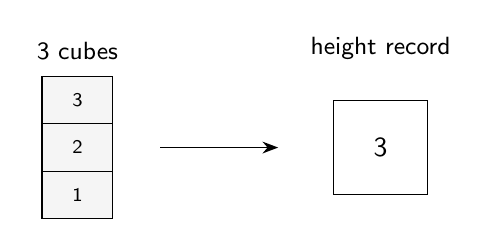
\begin{tikzpicture}[x=1mm,y=1mm,baseline=(current bounding box.center)]
  \foreach \h in {0,1,2} {
    \draw[fill=gray!8] (0,\h*6) rectangle (9,{(\h+1)*6});
    \node[font=\scriptsize] at (4.5,\h*6+3) {\number\numexpr\h+1\relax};
  }
  \node[anchor=south,font=\small] at (4.5,19) {3 cubes};
  \draw[-{Stealth[length=2mm]},line width=0.6pt] (15,9)--(30,9);
  \draw (37,3) rectangle (49,15);
  \node at (43,9) {3};
  \node[anchor=south,font=\small] at (43,19) {height record};
\end{tikzpicture}%
}
\newcommand{\routedemo}{%
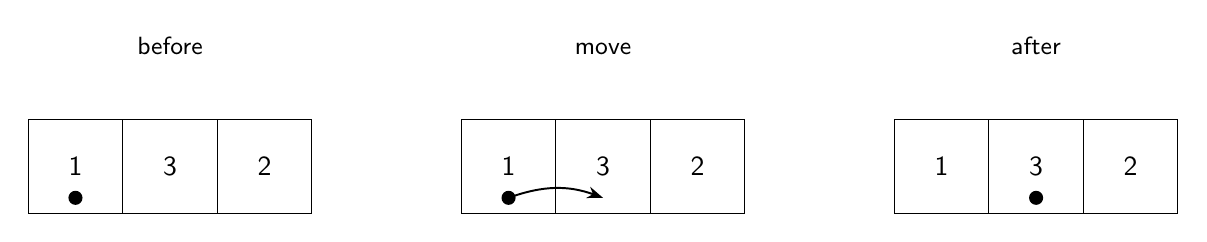
\begin{tikzpicture}[x=1mm,y=1mm,baseline=(current bounding box.center)]
  \foreach \x/\label/\marker in {0/before/0,55/move/0,110/after/1} {
    \foreach \j/\v in {0/1,1/3,2/2} {
      \draw (\x+\j*12,0) rectangle +(12,12);
      \node at (\x+\j*12+6,6) {\v};
    }
    \node[font=\small,anchor=south] at (\x+18,19) {\label};
    \ifnum\marker=1
      \node[fill=black,circle,inner sep=1.8pt] at (\x+18,2) {};
    \else
      \node[fill=black,circle,inner sep=1.8pt] at (\x+6,2) {};
    \fi
  }
  \draw[-{Stealth[length=2mm]},line width=0.7pt] (61,2) to[bend left=20] (73,2);
\end{tikzpicture}%
}

\begin{document}
In a city, each row and each column has one tower of every height: 1, 2, 3 for a 3-by-3 city, or 1, 2, 3, 4 for a 4-by-4 city. A number in a square records its tower's height.

\begin{center}\heightdemo\end{center}

\textbf{Problem 1:} Build one printed city at a time. Starting from that city each time, find different ways to change the heights at exactly four squares and still obey the city rule. Leave every other height as it was. Mark the changed squares in your final records. Which cities allow this? Can you change a city at fewer than four squares?

\vspace{2mm}
\begin{center}
\makebox[52mm]{A}\hspace{7mm}\makebox[52mm]{B}\hspace{7mm}\makebox[52mm]{C}
\par\vspace{1mm}
\makebox[52mm]{\city{4}{10}{\CityA}{0}}\hspace{7mm}%
\makebox[52mm]{\city{4}{10}{\CityB}{0}}\hspace{7mm}%
\makebox[52mm]{\city{3}{10}{\CityC}{0}}
\par\vspace{5mm}
\makebox[52mm]{\blankcity{4}{11}{0}}\hspace{7mm}%
\makebox[52mm]{\blankcity{4}{11}{0}}\hspace{7mm}%
\makebox[52mm]{\blankcity{3}{11}{0}}
\par\vspace{5mm}
\makebox[52mm]{\blankcity{4}{11}{0}}\hspace{7mm}%
\makebox[52mm]{\blankcity{4}{11}{0}}\hspace{7mm}%
\makebox[52mm]{\blankcity{3}{11}{0}}
\end{center}

\newpage
\textbf{Problem 2:} Build a city where both corner-to-corner diagonals also have one tower of every height. Try a 3-by-3 city and a 4-by-4 city. If a size cannot work, explain why.

\vspace{2mm}
\begin{center}
\begin{tabular}{@{}c@{\hspace{10mm}}l@{}}
\city{2}{14}{\DiagonalDemo}{1} &
\begin{tabular}{@{}l@{}}
dashed diagonal: 2, 2\\[3mm]
dotted diagonal: 1, 1
\end{tabular}
\end{tabular}
\end{center}

\vspace{5mm}
\begin{center}
\begin{tabular}{@{}c@{\hspace{4mm}}c@{}}
3 by 3 & 4 by 4\\[3mm]
\blankcity{3}{25}{1} & \blankcity{4}{25}{1}
\end{tabular}
\end{center}

\vfill
\rule{\textwidth}{0.25pt}\par\vspace{4mm}
\rule{\textwidth}{0.25pt}\par\vspace{4mm}
\rule{\textwidth}{0.25pt}\par\vspace{4mm}
\rule{\textwidth}{0.25pt}

\newpage
\textbf{Problem 3:} A roof route moves to a taller tower in a square that shares a side with the current square. It stops when no such move is left. Build each city and mark every square where a route can stop. Then design 3-by-3 or 4-by-4 cities with the fewest and most stopping squares you can. Build your designs on the table.

\begin{center}\routedemo\end{center}
\vspace{3mm}
\begin{center}
\begin{tabular}{@{}c@{\hspace{20mm}}c@{}}
D & E\\[3mm]
\city{3}{25}{\CityD}{0} & \city{3}{25}{\CityE}{0}
\end{tabular}
\end{center}

\vspace{4mm}
\begin{center}
\makebox[72mm]{fewest stopping squares}\hspace{10mm}\makebox[72mm]{most stopping squares}
\par\vspace{1mm}
\makebox[72mm]{\blankcity{3}{10}{0}}\hspace{10mm}\makebox[72mm]{\blankcity{3}{10}{0}}
\par\vspace{5mm}
\makebox[72mm]{\blankcity{4}{11}{0}}\hspace{10mm}\makebox[72mm]{\blankcity{4}{11}{0}}
\end{center}
\end{document}
